
%%%%%%%%%%%%%%%%%%%%%%%%%%%%%%%
\subsection{Approximate confidence distribution computing}
Approximate confidence distribution computing (ACDC) is a new take on likelihood-free inference within a frequentist setting. The development of this computational method for statistical inference hinges upon the modern notion of a {\it confidence distribution}, a special type of estimator which will be defined shortly. Through targeting this special distribution estimator rather than a specific likelihood or posterior distribution as in variational inference and approximate Bayesian inference, respectively, ACDC provides frequentist validation for inference in complicated settings with an unknown or intractable likelihood where dimension-reducing sufficient summary statistics may not even exist. This work demonstrates another example where confidence distribution estimators connect Bayesian and frequent inference, in the surprising context of computational methods for likelihood-free inference \cite{Xie2013, Thornton2022}.  
% \ST{ask Xie to cite sources}
	
% To clearly define an ACDC approach to computational inference, s

Let $x_{\rm obs} = \{x_1, \dots, x_n\}$ be an observed sample originating from a data-generating model that belongs to some complex parametric family $M_{\theta}$. Suppose the likelihood function is intractable (either analytically or computationally), but that this model is generative, i.e. given any $\theta \in \P$, we can simulate artificial data from $M_{\theta}$. Let $S_n(\cdot)$ be a summary statistic that maps the sample space into a smaller dimensional space and $r_{n}(\theta)$ be a data-dependent function on the parameter space. The simplest version of ACDC is the rejection algorithm labeled Algorithm 1 below, where $K_{\veps}(u) = \veps^{-1}K(u/ \veps)$ for a kernel function $K(\cdot)$ and $\veps$ is a small positive value, referred to as the {\it tolerance level}. 


	
% \vspace{-2mm}

% \noindent
%\scalebox{0.75}{
% \begin{minipage}{0.7\linewidth}

\noindent
\hrulefill
\vspace{-3mm}

\begin{algorithm}
\caption{Accept-reject approximate confidence distribution computing (ACDC)}\label{alg:rejACC} 
	\begin{tabbing}
	 1. Simulate $\theta_{1},\ldots,\theta_{N}\sim r_{n}(\theta)$; \\
	 For each $i=1,\ldots,N$, \\
	 \quad 2. Simulate $x^{(i)}=\{x_{1}^{(i)},\ldots,x_{n}^{(i)}\}$ from $M_{\theta_i}$;\\ 
	 \quad 3. Accept $\theta_{i}$ with probability $K_{\veps}(s^{(i)}-s_{\rm obs})$,\\ where $s_{{\rm obs}}=S_{n}(x_{\rm obs})$ and $ s^{(i)}=S_{n}(x^{(i)})$.
	\end{tabbing}
\end{algorithm}  

\vspace{-6mm}

\noindent
\hrulefill
%\end{minipage}
%}
\vspace{2mm}

The output of many iterations of Algorithm \ref{alg:rejACC} are potential parameter values, and %that generate artificial data that is similar to the observed data. 
these potential parameter values are draws from the probability density 
\begin{align} 
	q_{\veps}(\theta\mid s_{\rm obs})=
	\frac{\int_{ \cal S}r_{n}(\theta)f_n(s\mid\theta)K_{\veps}(s - s_{\rm obs})\,ds}{\int_{{\cal P} \times{\cal S}}r_{n}(\theta)f_n(s\mid\theta)K_{\veps}(s - s_{\rm obs})\,ds d\theta}.
\label{ACC_dist}
\end{align}
% and we denote the corresponding distribution by $Q_{\veps}(\theta\mid s_{\rm obs})$. 
Here, $f_n (  s \mid\theta)$ denotes the likelihood of the summary statistic, implied by the intractable likelihood of the data. Therefore $f_n (  s \mid\theta)$ is typically also intractable. We will refer to $f_n ( s \mid\theta)$ as an {\it s-likelihood} to emphasize that this is distinct from a traditional likelihood function $f_n (x_{obs} \mid\theta)$. We denote the cumulative distribution function corresponding to $q_{\veps}(\theta\mid s_{\rm obs})$ by $Q_{\veps}(\theta\mid s_{\rm obs})$. 

The main contribution of this paper is the establishment of a matching condition under which $Q_{\veps}(\theta\mid s_{\rm obs})$ is
an {\it approximate confidence distribution} for $\theta$ and can be used to derive various types of frequentist inferences. These conditions depend on the choice of $r_{n}(\theta)$ but are rather general and we present a strategy for choosing an appropriate data-dependent function in Section \ref{sec:largeSamp}. %This is a new perspective that has not yet been explored among the current literature of likelihood-free computing methods such as ABC. 
Practically, this new perspective allows the data to drive the algorithm in a way that can make it  more computationally effective than other existing likelihood-free approaches. Theoretically, this perspective establishes frequentist validation for inference from ACDC based upon general conditions that do not depend on the sufficiency of $s_{obs}$. 

Our justification for these practical and theoretical advantages of ACDC relies on the frequentist notion of a confidence distribution. Some background information on confidence distributions is presented next. To motivate the concept, first consider parameter estimation within a frequentist paradigm. We often desire that our estimators, whether point estimators or interval estimators, have certain properties such as unbiasedness or preform similarly under repeated, randomly sampling. A confidence distribution is an extension of this tradition in that it is a distribution estimate (i.e., it is a sample-dependent distribution function) that satisfies certain desirable properties. Following ~\cite{Xie2013} and ~\cite{Schweder2016}, we define a confidence distribution as follows:
	
{ {\it A sample-dependent function on the parameter space is a {\sc confidence distribution (CD)} for a parameter $\theta$ if 1) For each given sample, the function is a distribution function on the parameter space; 2) The function can provide valid confidence sets of all levels for $\theta$.} } 
	
A confidence distribution has a similar appeal to a Bayesian posterior in that it is a distribution function carrying much information about the parameter. A confidence distribution however, is a frequentist notion which treats the parameter as a fixed, unknown quantity and the sampling of data as the random event. %It is not a distribution of the parameter; rather, it 
A confidence distribution is a sample-dependent function that can be used to estimate the parameter of interest to quantify the uncertainty of the estimation. If $H_n(\cdot)$ is a CD for some parameter $\theta$, then one can simulate $\xi_{CD} \sim H_n{(\cdot)}$, conditional upon the observed data. We will refer to the random estimator $\xi_{CD} \sim H_n{(\cdot)}$ as a {\sc CD-random variable}. 

%\ST{[ADD: comments on how to read off confidence regions/intervals from a potentially multivariate CD?]}

The function $r_{n}(\theta)$ can be viewed as if it is a data-dependent prior. From a frequentist perspective, the data-dependent function $r_{n}(\theta)$ acts as an initial distribution estimate for $\theta$ and Algorithm~\ref{alg:rejACC} is a way to update this estimate in search of a better-preforming distribution estimate. This is analogous to any updating algorithm in point estimation requiring an initial estimate that is updated in search for a better-performing one (e.g., say, a Newton-Raphson algorithm or an expectation-maximization algorithm). Of critical concern in this perspective is ensuring that the data is not `doubly used' for inference. %We can avoid this problem by choosing 
An appropriate choice of the initial distribution estimate, $r_{n}(\theta)$, addresses this concern and a general strategy for choosing $r_n(\theta)$ is proposed later in  
%Under some conditions discussed later in 
Section \ref{sec:largeSamp}. %Algorithm \ref{alg:rejACC} can guarantee a distribution estimator for $\theta$ that follows the Repeated Sampling Principle. 
Therefore, this perspective asserts that $Q_{\veps}(\theta\mid s_{\rm obs})$ can be used for valid frequentist inference on $\theta$ (e.g., deriving confidence sets, $p$-values, etc.) %; however, Algorithm \ref{alg:rejACC} may 
even if it may sometimes not produce the most efficient estimator (i.e., may not produce the tightest confidence sets for all $\alpha\in (0,1)$ levels). % unless additional requirements are met. 
	
%In this paper, we demonstrate how the development of ACDC as a frequentist likelihood-free method is one of many examples in which CD theory provides a compelling inferential solution to a complicated problem that falls beyond the scope of conventional inferential arguments. When the target is inference for parameters of an intractable likelihood, or more generally, for parameters of generative models, this new perspective not only provides theoretical guarantees but also can greatly decrease computational costs compared to other likelihood-free methods. 

\subsection{Related work on Approximate Bayesian computing (ABC)}  
Approximate Bayesian computation (ABC)
refers to a family of computing algorithms to approximate posterior densities of $\btheta$ by bypassing direct likelihood evaluations \citep[cf.][]{% Rubin1984,Tavare1997,
Csillery2010,
Cameron2012,
Peters2012}.
The target of an ABC algorithm is the posterior distribution rather than a confidence distribution. 
A simple rejection sampling ABC proceeds in the same manner as Algorithm~\ref{alg:rejACC}, but it replaces $\theta_1, \ldots, \theta_N \sim r_{n}(\theta)$ with $\theta_1, \ldots, \theta_N \sim  \pi(\theta)$, a pre-specified prior distribution for $\theta$, in Step 1. %Here, $\pi(\theta)$ is a pre-specified prior distribution on $\theta$. 
In this article, we view ABC as a special case of ACDC where $r_{n}(\theta) = \pi(\theta)$.
% , a prior distribution on $\theta$.
The simple rejection sampling ABC is computationally inefficient. Some advanced computing techniques have been used to improve the simple ABC approach. One of such advanced algorithms that is comparable to Algorithm \ref{alg:rejACC} is the  an importance sampling version of ABC described in
Algorithm \ref{alg:ISABC}, where the $r_{n}(\theta)$ from Algorithm \ref{alg:rejACC} is treated as a reference distribution %that is used 
to facilitate and improve ABC computing efficiency.
% presents an importance sampling approach to ABC. % as an adaptation of Algorithm \ref{alg:rejACC} that incorporates the additional prior assumption.


\noindent
\hrulefill

\vspace{-3mm}
\begin{algorithm}
\caption{Importance sampling ABC (IS-ABC)} \label{alg:ISABC}
	\begin{tabbing}
	 1. Simulate $\btheta_{1},\ldots,\btheta_{N}\sim r_{n}(\btheta)$. \\
	 For each $i=1,\ldots,N$, \\
	 \quad 2. Simulate $\bx^{(i)}=\{x_{1}^{(i)},\ldots,x_{n}^{(i)}\}$ from $M_{\btheta}$.\\ 
	 \quad 3. Accept $\btheta_{i}$ with probability $K_{\veps}(s^{(i)}-s_{\rm obs})$,\\ 
	 \quad where $s_{\rm obs}= S_{n}(\bx_{\rm obs})$ and $ s^{(i)}=S_{n}(\bx^{(i)})$, and assign \\ \quad importance weights $w(\theta_i)=\pi(\theta_i)/r_{n}(\theta_i)$.
	\end{tabbing}
\end{algorithm}  

\vspace{-6mm} 

\noindent
\hrulefill

%The typical goal of %A common assertion of 
The theoretical argument behind an approximate Bayesian inference (either using the simple rejection sampling ABC or IS-ABC) %Algorithm~\ref{alg:ISABC})
 depends upon $q_{\veps}(\theta\mid s_{\rm obs})$ converging to the posterior, $p(\theta \mid x_{obs}) = {\pi(\theta) f_n ( x_{obs} \mid\theta)}\big/{\int \pi(\theta) f_n ( x_{obs} \mid\theta)
d \theta }$, as the tolerance level approaches zero; c.f., e.g.~\cite{Marin2011} and \cite{Beaumont2019}. However, it is well-known that the quality of this approximation depends not only on the size of $\veps$ (and choice of prior) but, also importantly, upon the choice of summary statistic. If $s_{obs}$ is not sufficient (as is gerenally the case in applications of ABC), then the s-likelihood $f_n (s_{obs} \mid\theta)$ can be very different from the likelihood of the data $f_n ( x_{obs} \mid\theta)$ and thus $q_{\veps}(\theta\mid s_{\rm obs})$ can be a very poor approximation to $p(\theta\mid x_{obs})$, even as $\veps$ approaches zero and $n \rightarrow \infty$.

For example, consider using Algorithm \ref{alg:rejACC} with two different choices of summary statistic, the sample mean or median, for estimating the location parameter of a random sample ($n=100$) from $Cauchy(10, 0.55)$. If we suppose $r_n(\theta) \propto 1$, then our algorithm is not data-driven and $r_n(\theta)$ instead acts as an uninformative prior. Hence this example corresponds to an accept-reject version of ABC algorithm. 
Figure~\ref{fig:ACC} shows $q_{\veps}(\theta\mid s_{\rm obs})$ for each choice of summary statistic (black lines) where $\veps = 0.005$. 
%Figure \ref{fig:ACC} shows that the distribution estimator resulting from this application of Algorithm~\ref{alg:rejACC} with either the mean or median as the summary statistic (solid black lines) does not converge to the target
The posterior distribution (solid gray lines) does not match well with either approximate ABC posterior distribution $q_{\veps}(\theta\mid s_{\rm obs})$ because only the entire data vector itself is sufficient in this example. This example demonstrates how a strictly ABC approach that targets $p(\theta \mid x_{obs})$ can produce inconsistent results and even misleading inferential conclusions.

\begin{figure}
\centering
\caption{{\it The gray curves below represent the target posterior distribution (gray lines), $p(\theta \mid \bx)$, for an $n=100$ IID sample from $Cauchy(\theta=10,0.55)$. The curves in black represent  $q_{\veps}(\theta \mid s_{obs})$ for two different summary statistics, $S_{n_1} = Median(x)$ (left) and $S_{n_2} = \bar{x}$ (right). In each case $\veps = 0.005$.} }\label{fig:ACC}
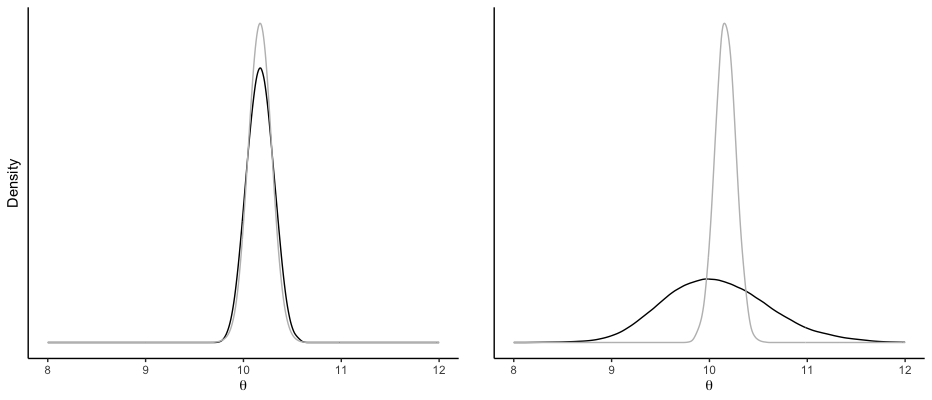
\includegraphics[
width = .9\linewidth, height=5.2cm,
]{Cauchy_ABC_fig_n100.png}
\end{figure}	


%%%%%%%%%%%%%%%%%%%%%%%%%%%%%%%%%%%%%%%%%%%%%%%%%%%%%%%%%%%%%%%%%%%%%%%%
To quote \cite[]{marquette_statistics_2021}: ``the choice of the summary statistic is essential to ensure ABC produces a reliable approximation to the true posterior distribution." Much of the current literature on ABC methods is appropriately oriented towards the selection and evaluation of the summary statistic. 
%\ST{something about approximate sufficient summary stats, finding optimal selection of summary stats}.
%The main focus of the recent ABC literature has been on the selection and evaluation of summary statistics, including a Royal Statistical Society Read Paper (Fearnhead and Prangle, 2012) that set a reference and gave prospective developments in the discussion section.
%marquette_statistics_2021 Marquette, Jean-Baptiste. 2018. Statistics for Astrophysics : Bayesian Methodology. Les Ulis: EDP Sciences.
The theoretical justification for inference from ACDC on the other hand, does not require an optimal selection of $S_n$. Although less informative summary statistics may lead to less efficient CDs, the validity of the inferential conclusions can remain intact even for less informative (and non-sufficient) summary statistics. (See Sections \ref{sec:main} and \ref{sec:ex}.)

%In this article, we establish conditions under which Algorithm \ref{alg:rejACC} yields valid likelihood-free inference with respect to the Repeated Sampling Principle, something that is generally not the focus of current research on likelihood-free methods. \ST{exception of approximate Bayesian inference conferences} Furthermore, a theoretical result presented in Section \ref{sec:thms} specifies general conditions under which Algorithm \ref{alg:rejACC} can be used to conduct inference in settings that extend beyond the reaches of conventional large sample arguments.  

The large sample theoretical results presented in Section \ref{sec:largeSamp} specify conditions under which Algorithm \ref{alg:rejACC} produces an asymptotically normal confidence distribution. These results are similar to those in~\cite{Li2017} % \ST{[ask Wentao if other citations should be included here]} 
but our work is distinct because we do not target an approximation to a posterior distribution. Instead, the theoretical results in this section of our paper focus on the properties and performance of ACDC inherited through its connection to CDs. Additionally, in Section \ref{sec:largeSamp} we propose a regression-adjustment technique based on that of \cite{Li2017} and \cite{Blum2010}. This post-processing step for ACDC is applied to Algorithms \ref{alg:rejACC} and \ref{alg:ISABC} in Section \ref{sec:ex} to improve the accuracy of the CDs.

%The main goal of this article is to present the idea that the continued study of likelihood-free methods can benefit from the incorporation of confidence distribution theory. To this end, and for the ease of presentation, we mainly focus on Algorithm \ref{alg:rejACC}, although we compare the performance of Algorithm \ref{alg:rejACC} with that of Algorithm \ref{alg:ISABC} in Section \ref{sec:ex}. 

Computationally, the numerical studies in Section~\ref{sec:ex} also suggest that 
accept-reject ACDC %Algorithm~\ref{alg:rejACC} 
is more stable than the IS-ABC %Algorithm~\ref{alg:ISABC}, although 
even when both approaches utilize the same data-driven function $r_{n}(\theta)$. This difference in performance is due to the fact that the importance weights  $w(\theta)=\pi(\theta)/r_{n}(\theta)$ in in IS-ABC %Algorithm~\ref{alg:ISABC}  
can fluctuate greatly causing numerical instability in the generated parameter values. %and are numerically unstable. 
%Nevertheless, t
The steep computing cost associated with the generative model is an expansive area of current research on likelihood-free methods including adaptations that decrease the computing cost of approximate Bayesian methods %include 
such as MCMC methods \cite[]{marjoram2003markov} and sequential Monte Carlo techniques\cite[]{Sisson2007}. Although an exploration of these adaptations is beyond the scope of this paper, we expect that many of these approaches can be readily applied to improve the computational performance of ACDC as well. %Furthermore, t
The numerical examples in Section \ref{sec:ex} 
demonstrate how accept-reject ACDC 
%illustrate some cases in which 
%Algorithm \ref{alg:rejACC} 
accepts more simulations than IS-ABC
%Algorithm \ref{alg:ISABC}, 
suggesting that merely incorporating $r_n(\theta)$ as a data-dependent proposal function is not computationally preferable. 
%may not always be computationally preferable in comparison to an accept-reject version of ACDC. 

%$Q_{\veps}$ from Algorithm \ref{alg:rejACC} may share the same limiting distribution resulting from ABC. However, because $r_n(\theta)$ concentrates more probability mass around the target value, $\theta_0$, ACDC may accept more simulations than the Bayesian counterpart and can therefore be regarded as more computationally efficient. 

%Furthermore, even an importance sampling version of ABC~\cite[]{Fearnhead2012} where the proposal matches $r_n(\theta)$, given in Algorithm~\ref{alg:ISABC}, may under-perform in comparison to Algorithm \ref{alg:rejACC}  %which assigns equal weights to the output sample. Algorithm~\ref{alg:ISABC} because highly skewed importance weights may result in higher Monte Carlo variance. This issue could increase in severity with $n$ since the sample weight, $\pi(\theta)/r_n(\theta)$, is unbounded as $r_n(\theta)$ is increasingly peaked. Related discussions and controlling techniques for ABC can be found in \cite{Li2016}. The numerical examples in Section \ref{sec:discuss} of this article demonstrate this issue.
%%%%%%%%%%%%%%%%%%%%%%%%%%%%%%%%%%%%%%%%%%%%%%%%%%%%%%%%%%%%%%%%%%%%%%%%

	
\subsection{Notation and outline of topics}
In addition to the notation from the introduction, throughout the remainder of paper we will use the following notation. The observed data is $x_{\rm obs} \in \mathscr{X} \subset \mathbb{R}^n$, the summary statistic is a mapping $S_n: \mathscr{X} \rightarrow {\cal S} \subset \mathbb{R}^{d}$ and the observed summary statistic is $s_{\rm obs} = S_n(x_{\rm obs})$. The parameter of interest is $\theta \in \P \subset \mathbb{R}^p$ with $p \leq d < n$; i.e. the number of unknown parameters is no greater than the number of summary statistics and the dimension of the summary statistic is smaller than the dimension of the data. If some function of $S_n$ is an estimator for $\theta$, we will denote this function by $\hat{\theta}_S$. 

%\ST{In this article, when we refer to Algorithm \ref{alg:rejACC}, we are referencing explicitly a frequentist approach to likelihood-free inference. The abbreviation ACDC is used to refer to a broader class of variations on Algorithm \ref{alg:rejACC} that still utilize $r_n(\theta)$ and target a confidence distribution. 
%but may include specific applications in a Bayesian setting. References to Algorithm \ref{alg:ISABC} on the other hand, point to a particular importance sampling, Bayesian adaptation of Algorithm \ref{alg:rejACC} that assumes an uninformative prior for $\theta$ but still utilizes $r_n(\theta)$ and targets a confidence distribution. }

The next section presents the core theoretical result of this paper %our first main theoretical result 
which establishes a necessary condition for ACDC methods to produce a valid CD, thereby %it can be used as a 
establishing ACDC as a likelihood-free method that provides valid frequentist inference. 
% validating inference from likelihood-free methods.
%\ST{The theoretical content from this section begins to lay the foundation for our larger theoretical argument in favor of orienting likelihood-free inference as a search for a CD.} 
Section \ref{sec:largeSamp} presents general large sample conditions for ACDC that produce asymptotic CDs and establishes precise conditions for an appropriate choice of the data-dependent function $r_n(\theta)$. Section \ref{sec:ex} contains two numerical examples that verify the inferential conclusions of ACDC and illustrate the computational advantages of this data-driven algorithm. Section \ref{sec:discuss} concludes with a brief discussion. All proofs for Sections \ref{sec:thms} and \ref{sec:largeSamp} are contained in the Appendix (and supplementary material). 


